\section{Elektronik-Entwicklungsumgebung für Layout und Leiterplatten \enquote{Altium}} \label{sec:6.1}
\enquote{Altium Designer} ist eine Software zum Entwickeln und Designen von elektronischen Leiterplatten (engl. PCB).\\
In unserem Fall wurde die Version 13.3 verwendet. 
\begin{figure} [H]
	\centering
	
\includegraphics[width=0.8\textwidth]{img/Grundlagen/Altium/ad_logo.png}
	\caption[Logo von \enquote{Altium Designer}]{Logo von \enquote{Altium Designer}\footnotemark}
	%http://www.altium.com/resources/images/media-release/ad_logo.png
	\label{fig:6.1.1}
\end{figure}
\footnotetext{http://www.altium.com/resources/images/media-release/ad\_logo.png,\\Zugriff: 16.02.2017}
Für jedes neues \enquote{PCB}-Projekt muss eine \enquote{Schematic}-Datei und eine \enquote{PCB}-Datei angelegt werden.

\newpage
\section{Filterberechnungstool \enquote{FilterPro}}\label{sec:6.2}
\enquote{FilterPro} ist eine Software zur Berechnung aktiver Filter verschiedener Art.
Diese Software wird von dem Hersteller \enquote{Texas Instruments} gratis zur Verfügung gestellt.\\
In unserem Fall wurde die Version 3.1.0 verwendet. 
\begin{figure} [H]
	\centering
	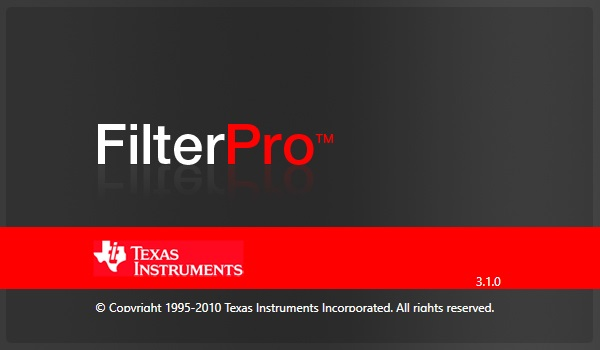
\includegraphics[width=0.65\textwidth]{img/VerwendeteTools/FilterPro.jpg}
	\caption[Logo von \enquote{FilterPro}]{Logo von \enquote{FilterPro}}
	%Screenshot-Macsek Zugriff: 11.03.2017
	\label{fig:6.2.1}
\end{figure}
Es wurden alle verwendeten Frequenzweichen vor Entwickeln der Leiterplatten in diesem Programm berechnet.
